%%%%%%%%%%%%%%%%%%%%%%%%%%%%%%%%%%%%%%%%%
% Beamer Presentation
% LaTeX Template
% Version 1.0 (10/11/12)
%
% This template has been downloaded from:
% http://www.LaTeXTemplates.com
%
% License:
% CC BY-NC-SA 3.0 (http://creativecommons.org/licenses/by-nc-sa/3.0/)
%
%%%%%%%%%%%%%%%%%%%%%%%%%%%%%%%%%%%%%%%%%

%----------------------------------------------------------------------------------------
%	PACKAGES AND THEMES
%----------------------------------------------------------------------------------------

\documentclass{beamer}

\usepackage{minted}
\usepackage{float}
\usepackage{caption}

\mode<presentation> {

% The Beamer class comes with a number of default slide themes
% which change the colors and layouts of slides. Below this is a list
% of all the themes, uncomment each in turn to see what they look like.

%\usetheme{default}
%\usetheme{AnnArbor}
%\usetheme{Antibes}
%\usetheme{Bergen}
%\usetheme{Berkeley}
%\usetheme{Berlin}
%\usetheme{Boadilla}
%\usetheme{CambridgeUS}
%\usetheme{Copenhagen}
%\usetheme{Darmstadt}
%\usetheme{Dresden}
%\usetheme{Frankfurt}
%\usetheme{Goettingen}
%\usetheme{Hannover}
%\usetheme{Ilmenau}
%\usetheme{JuanLesPins}
%\usetheme{Luebeck}
%\usetheme{Madrid}
%\usetheme{Malmoe}
%\usetheme{Marburg}
%\usetheme{Montpellier}
%\usetheme{PaloAlto}
%\usetheme{Pittsburgh}
%\usetheme{Rochester}
%\usetheme{Singapore}
%\usetheme{Szeged}
\usetheme{Warsaw}

% As well as themes, the Beamer class has a number of color themes
% for any slide theme. Uncomment each of these in turn to see how it
% changes the colors of your current slide theme.

%\usecolortheme{albatross}
%\usecolortheme{beaver}
%\usecolortheme{beetle}
%\usecolortheme{crane}
%\usecolortheme{dolphin}
%\usecolortheme{dove}
%\usecolortheme{fly}
%\usecolortheme{lily}
%\usecolortheme{orchid}
%\usecolortheme{rose}
%\usecolortheme{seagull}
%\usecolortheme{seahorse}
%\usecolortheme{whale}
%\usecolortheme{wolverine}

%\setbeamertemplate{footline} % To remove the footer line in all slides uncomment this line
\setbeamertemplate{footline}[page number] % To replace the footer line in all slides with a simple slide count uncomment this line

\setbeamertemplate{navigation symbols}{} % To remove the navigation symbols from the bottom of all slides uncomment this line
}

\usepackage{graphicx} % Allows including images
\usepackage{booktabs} % Allows the use of \toprule, \midrule and \bottomrule in tables

%----------------------------------------------------------------------------------------
%	TITLE PAGE
%----------------------------------------------------------------------------------------

\title{Razvoj SUPB z integracijo v programski jezik Python} % The short title appears at the bottom of every slide, the full title is only on the title page

\author{Janez Sedeljšak
\\ Mentor: doc. dr. Boštjan Slivnik
\\ Somentor: asist. dr. Marko Poženel
} % Your name
\institute[UL FRI] % Your institution as it will appear on the bottom of every slide, may be shorthand to save space
{
Univerza v Ljubljani, Fakulteta za računalništvo in informatiko \\ % Your institution for the title page
\medskip
\textit{js0578@student.uni-lj.si} % Your email address
}
\date{\today} % Date, can be changed to a custom date

\begin{document}

\begin{frame}
\titlepage % Print the title page as the first slide
\end{frame}

%----------------------------------------------------------------------------------------
%	PRESENTATION SLIDES
%----------------------------------------------------------------------------------------

%------------------------------------------------
\section{Uvod} % Sections can be created in order to organize your presentation into discrete blocks, all sections and subsections are automatically printed in the table of contents as an overview of the talk
%------------------------------------------------

\subsection{Motivacija}
\begin{frame}
\frametitle{Motivacija}
    \begin{itemize}
        \item{Spoznati delovanje podatkovnih baz}
        \begin{itemize}
            \item{Izogib uporabi anti-vzorcev}
            \item{Boljša implementacija podatkovnega sloja}
        \end{itemize}
    \end{itemize}
    \vfill
    \begin{itemize}
        \item{Razvoj minimalističnega SUPB za programski jezik Python:}
        \begin{itemize}
            \item{SUPB na nivoju programskega jezika C++}
            \item{Indeksiranje z uporabo B+ dreves}
            \item{Intuitiven način komunikacije s podatkovno bazo}
            \item{Izhodišče sta MySQL in SQLite}
        \end{itemize}
    \end{itemize}
\end{frame}

\section{Implementirana rešitev}

    \subsection{Arhitektura rešitve Graphenix}
    \begin{frame}
    \frametitle{Arhitektura rešitve Graphenix}
        \centering
        \includegraphics[height=4.5cm]{graphenix_structure.png}
    \end{frame}

    \subsection{Mehanizem za shranjevanje}
    \begin{frame}
    \frametitle{Struktura shranjenih podakov}
        \centering
        \includegraphics[height=4.5cm]{struktura_entitet.png}
    \end{frame}

    \begin{frame}
    \frametitle{Indeksiranje z uporabo B+ drevesa}
    \begin{itemize}
        \item Implementacija s pomočjo programskega jezika C++
        \item Shranjevanje strukture v binarni datoteki
        \item Uporaba ``generikov`` za različne podatkovne tipe (nizi, cela števila, realna števila, povezave)
        
        \centering
        \includegraphics[height=3cm]{Bplustree.png}
    \end{itemize}
    \end{frame}

\section{Predstavitev delovanja}
    \subsection{Definiranje sheme}
    \begin{frame}[fragile]
    \frametitle{Definiranje sheme}
    \footnotesize
        \begin{minted}{python}
class User(gx.Model):
    name = gx.Field.String(size=100)
    tasks = gx.Field.VirtualLink("user")
    sent = gx.Field.VirtualLink("sender")
    received = gx.Field.VirtualLink("receiver")
    
class Task(gx.Model):
    content = gx.Field.String(size=100)
    user = gx.Field.Link()
    
class Message(gx.Model):
    content = gx.Field.String(size=50)
    date = gx.Field.DateTime()
    sender = gx.Field.Link().as_index()
    receiver = gx.Field.Link().as_index()
        \end{minted}
    \end{frame}

    \subsection{Poizvedovanje}
    \begin{frame}[fragile]
    \frametitle{Poizvedovanje}
    \footnotesize
    \begin{minted}{python}
# uporabniki urejeno po imenu - padajoče
_, view = User.order(User.name.desc()).all()

# uporabniki in njihove naloge
_, view = User.link(tasks=Task).all()

# število sporočil in datum zadnjega sporočila po uporabnikih
counts = Message.agg(by=Message.sender, 
    count=gx.AGG.count(), latest=gx.AGG.max(Message.date))
    
    \end{minted}
    \end{frame}

    \subsection{Vgnezdne poizvedbe}
    \begin{frame}[fragile]
    \frametitle{Vgnezdne poizvedbe}
    \begin{block}{Nabor uporabnikov, njihovih nalog in prejetih sporočil, kjer na sporočila vežemo še pošiljatelja}
    \footnotesize
    \begin{minted}{python}
_, view = User.link(
    tasks=Task.limit(3), 
    received=Message.link(sender=User)
).filter(User.name.iregex('john.*')).all()
        \end{minted}
    \end{block}

    \footnotesize
    \begin{minted}{JSON}
{
    "name": "John Doe",
    "tasks": [
        {"content": "Finish the diploma"},
    ],
    "received": [
        {"content": "Hello", "sender": {}},
    ]
}
    \end{minted}
    \end{frame}
    
\section{Analiza delovanja}
    \subsection{Vstavljanje}
    \begin{frame}
    \frametitle{Vstavljanje zapisov}
    \begin{figure}
        \begin{minipage}[t]{0.45\textwidth}
            \centering
            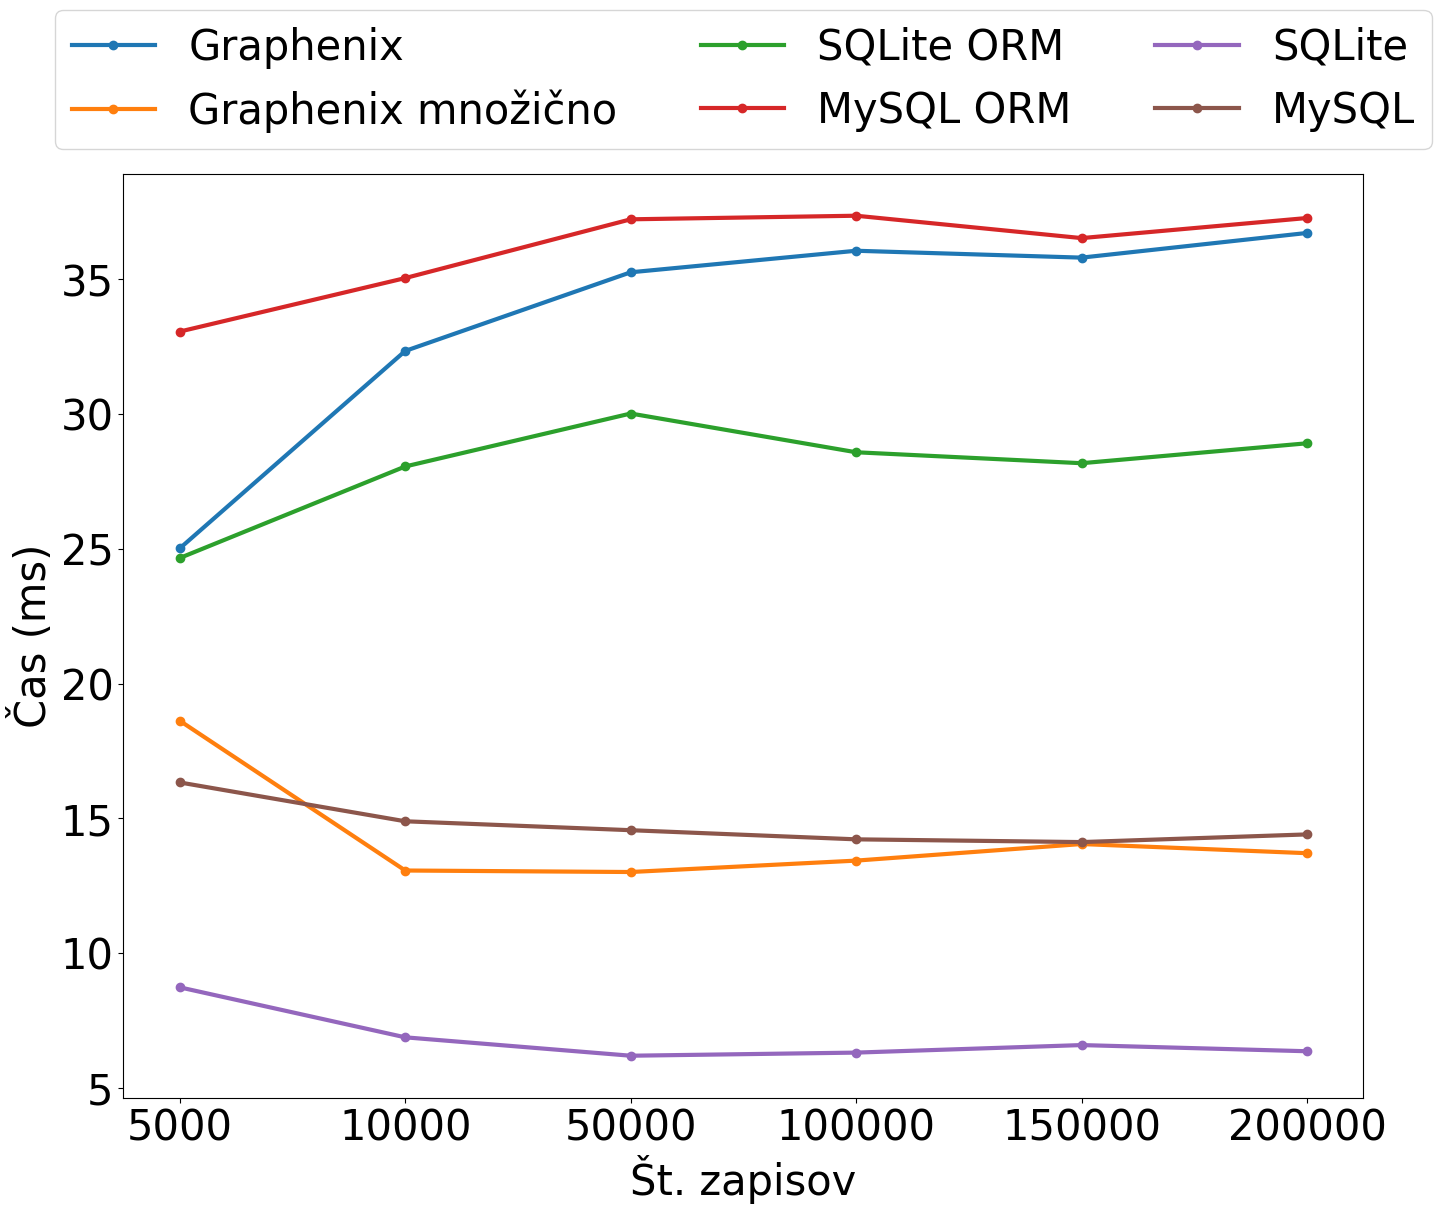
\includegraphics[height=4cm]{singleinsert.png}
            \caption*{Množično vstavljanje podatkov.}
        \end{minipage}
        \hfill
        \begin{minipage}[t]{0.45\textwidth}
            \centering
            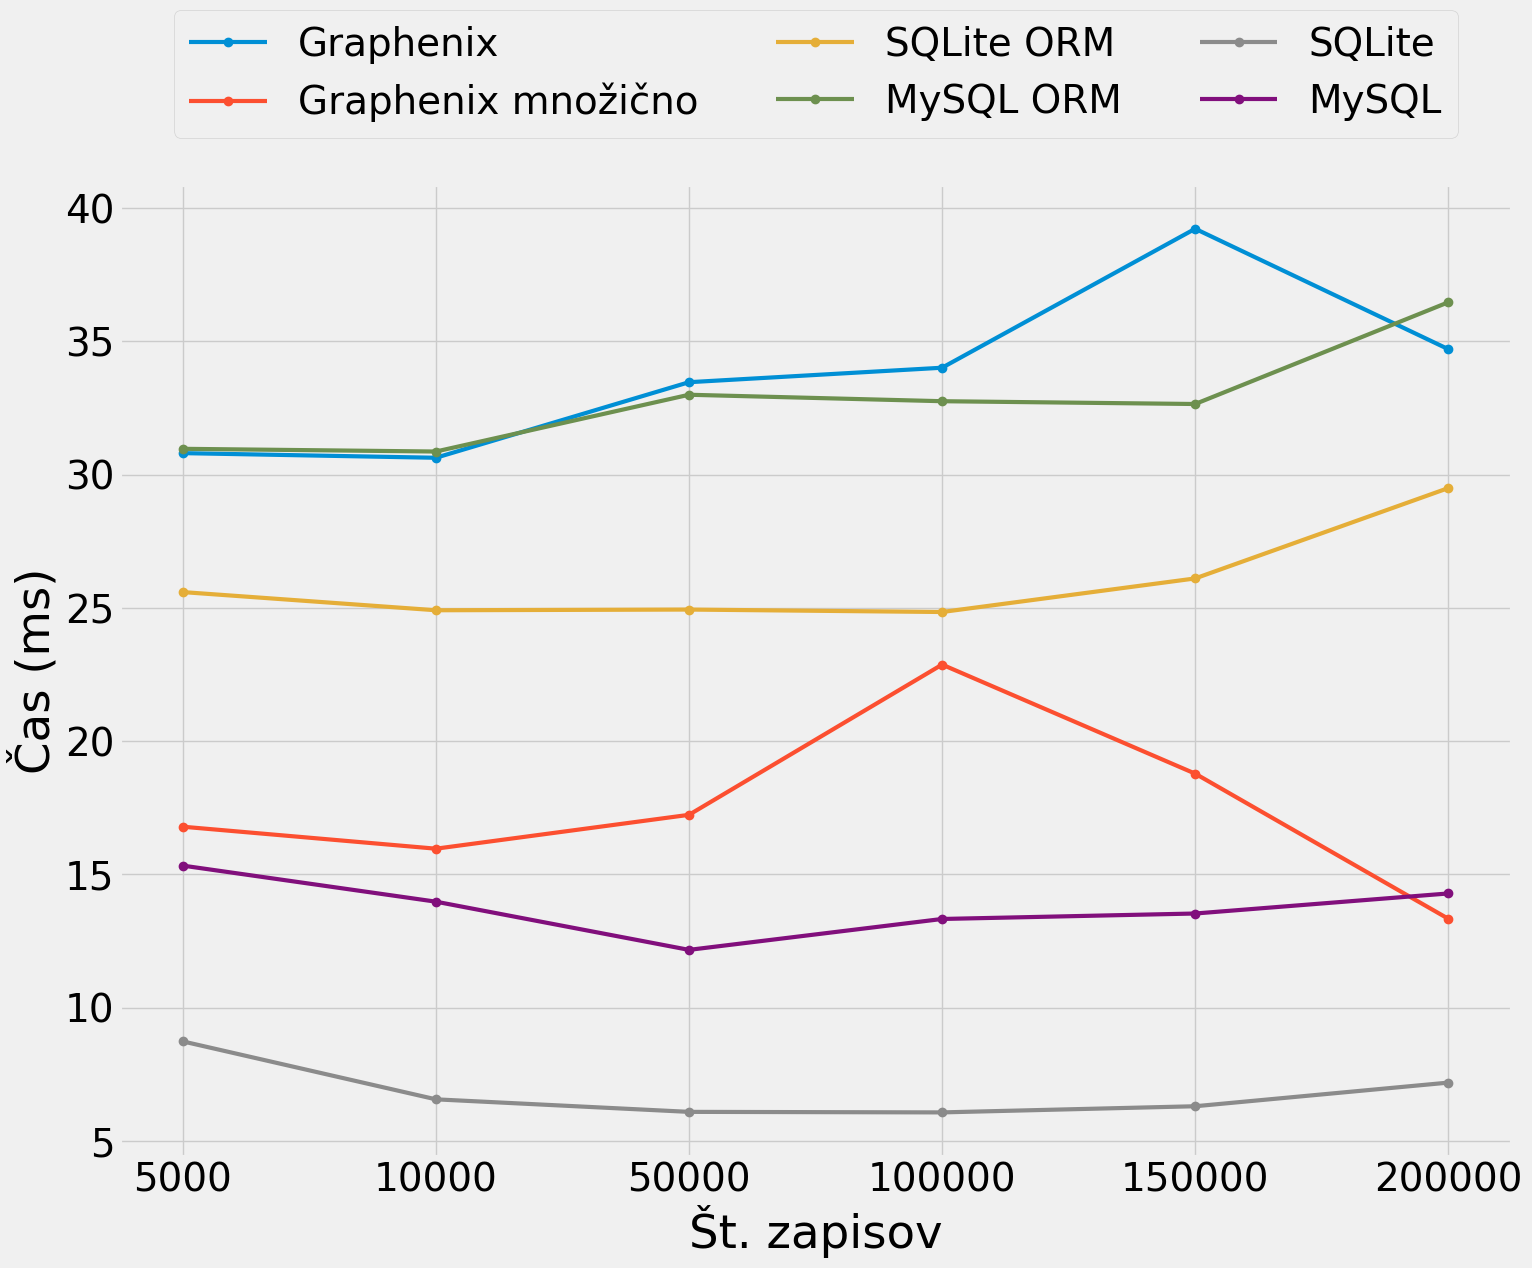
\includegraphics[height=4cm]{indexinsert.png}
            \caption*{Vstavljanje z dodatnim indeksiranim poljem.}
        \end{minipage}
    \end{figure}
\end{frame}

    \subsection{Poizvedovanje}
    \begin{frame}
        \frametitle{Poizvedovanje}
        \begin{figure}
            \begin{minipage}[t]{0.45\textwidth}
                \centering
                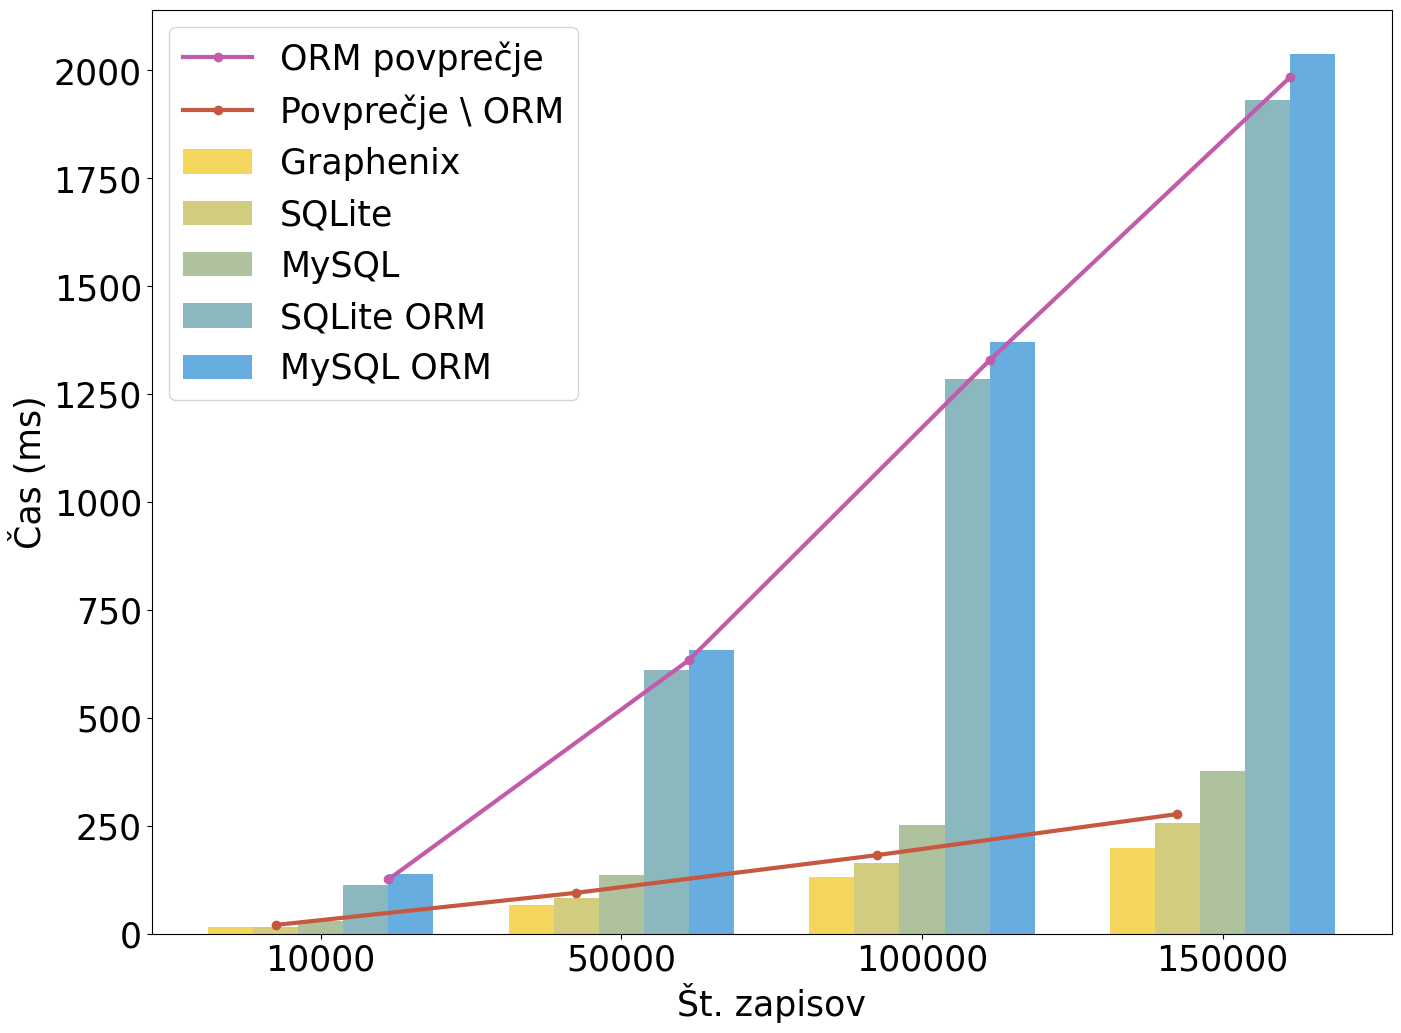
\includegraphics[height=4cm]{singleread.png}
                \caption*{Branje brez dodatnih parametrov znotraj poizvedbe.}
            \end{minipage}
            \hfill
            \begin{minipage}[t]{0.45\textwidth}
                \centering
                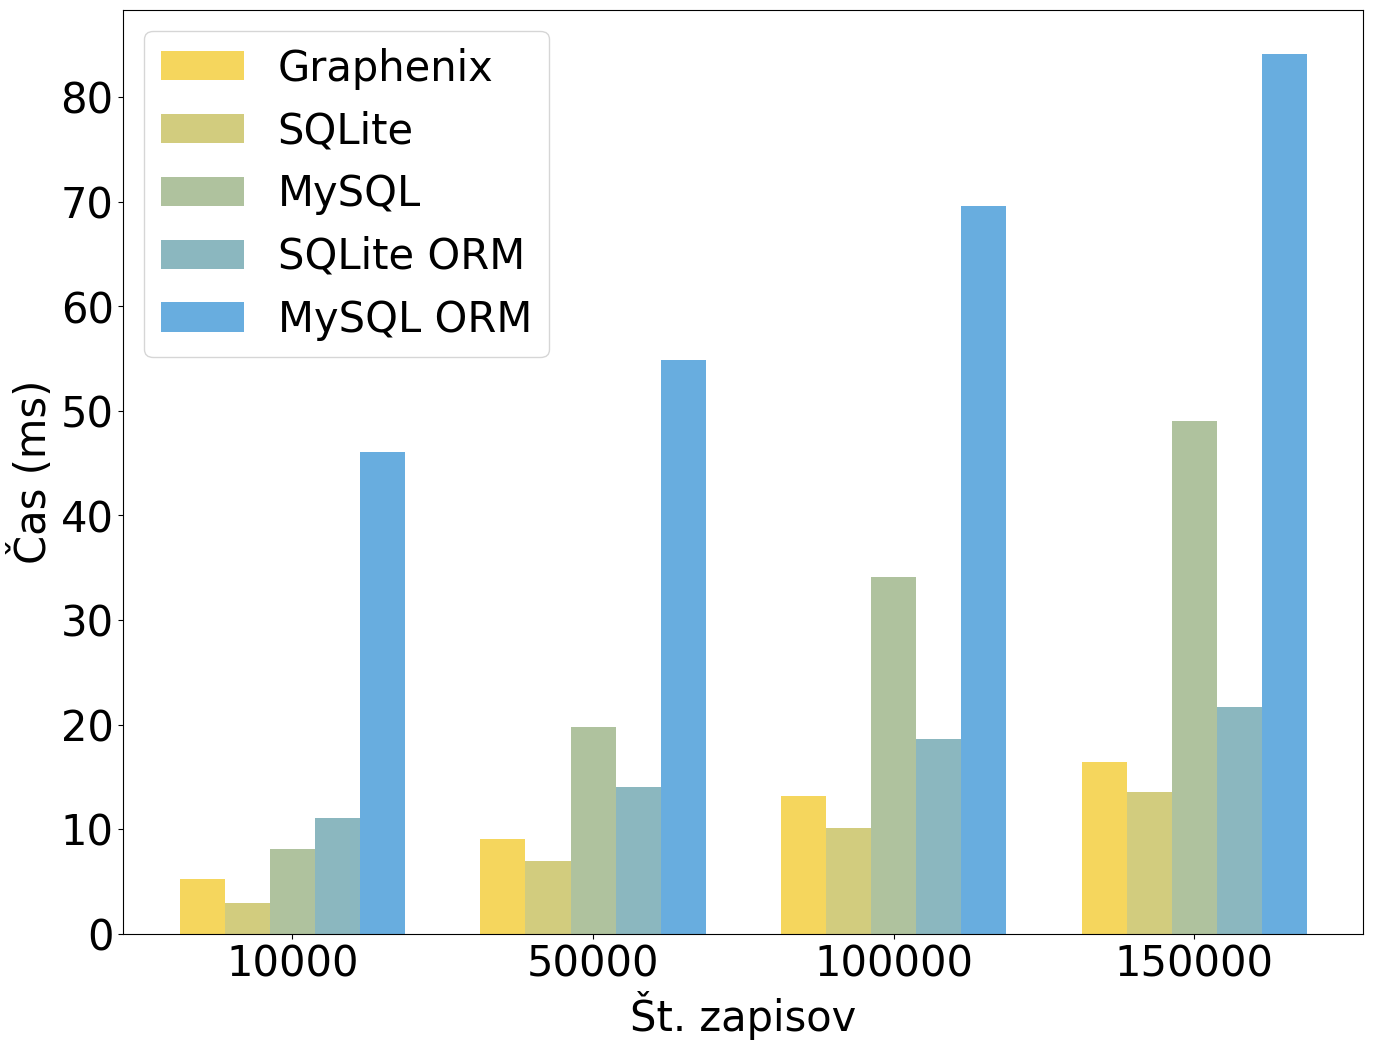
\includegraphics[height=4cm]{queryread.png}
                \caption*{Branje z omejitvami - prvih 500 uporabnikov + filtriranje + urejanje.}
            \end{minipage}
        \end{figure}
    \end{frame}

    \subsection{Uporaba indeksiranja}
    \begin{frame}
        \frametitle{Indeksiranje pred in po optimizaciji ($10^5$ zapisov)}
        \begin{figure}
            \begin{minipage}[t]{0.45\textwidth}
                \centering
                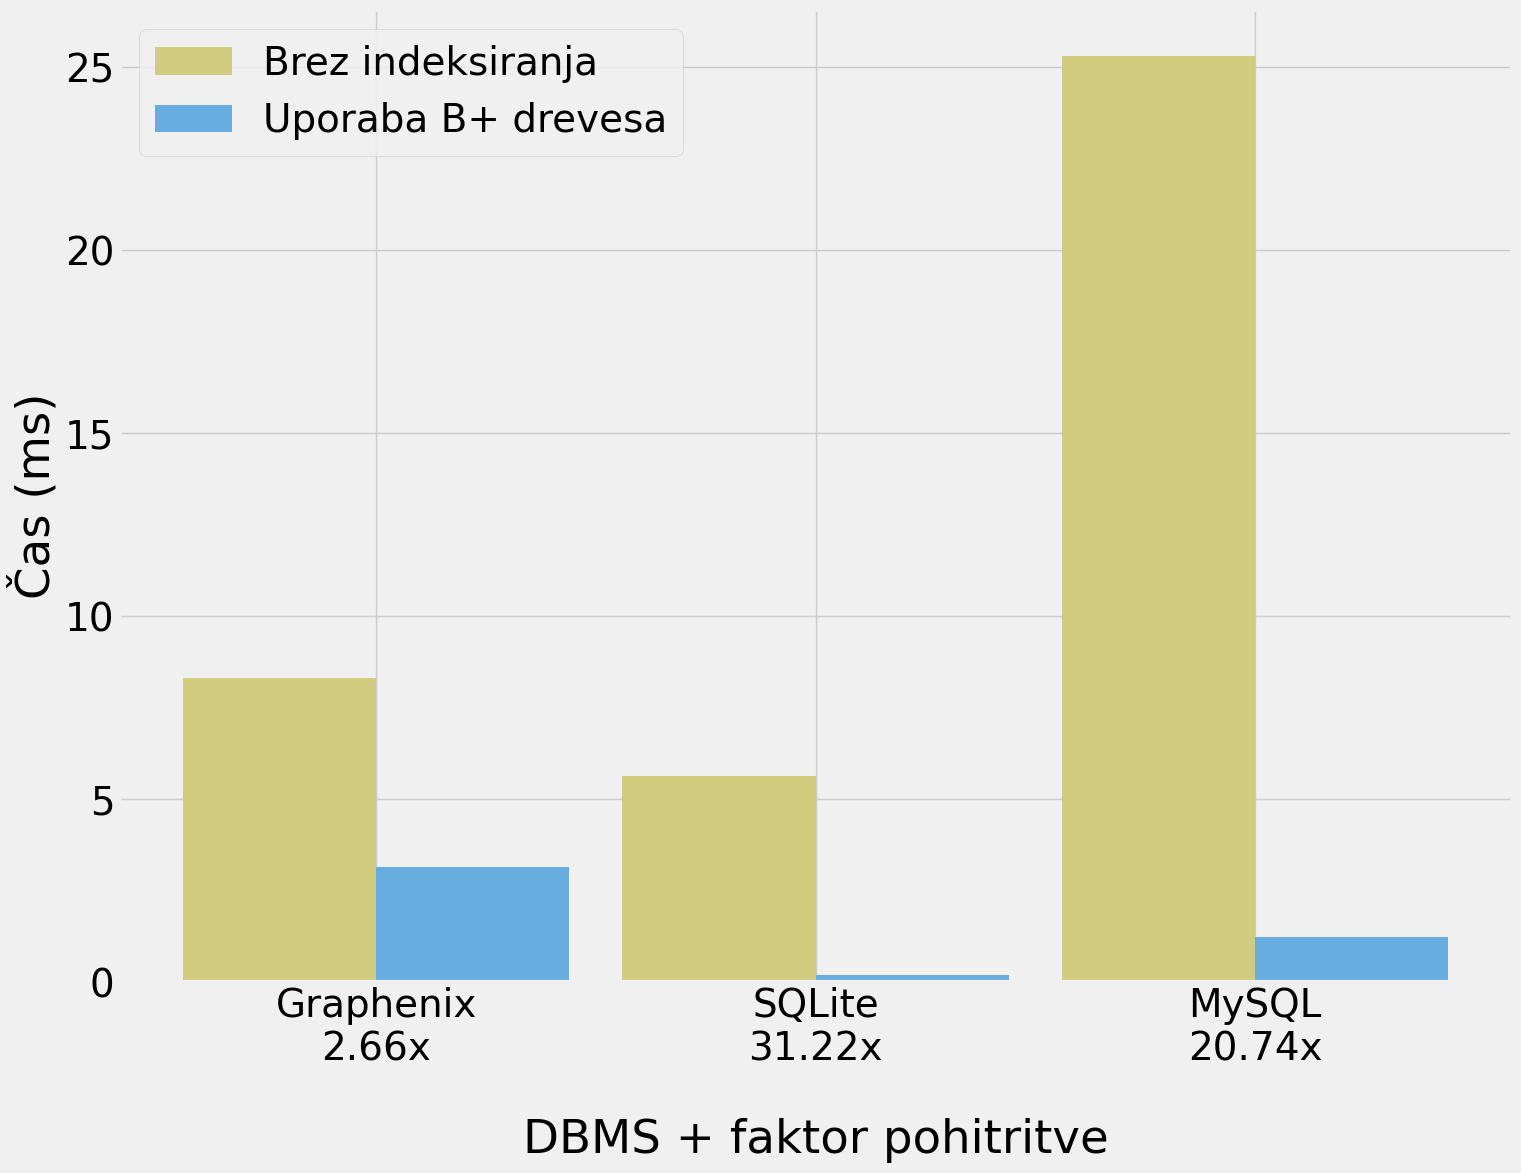
\includegraphics[height=4cm]{indexing_speedup_100000.png}
                \caption*{Pohitritve s pomočjo indeksiranja.}
            \end{minipage}
            \hfill
            \begin{minipage}[t]{0.45\textwidth}
                \centering
                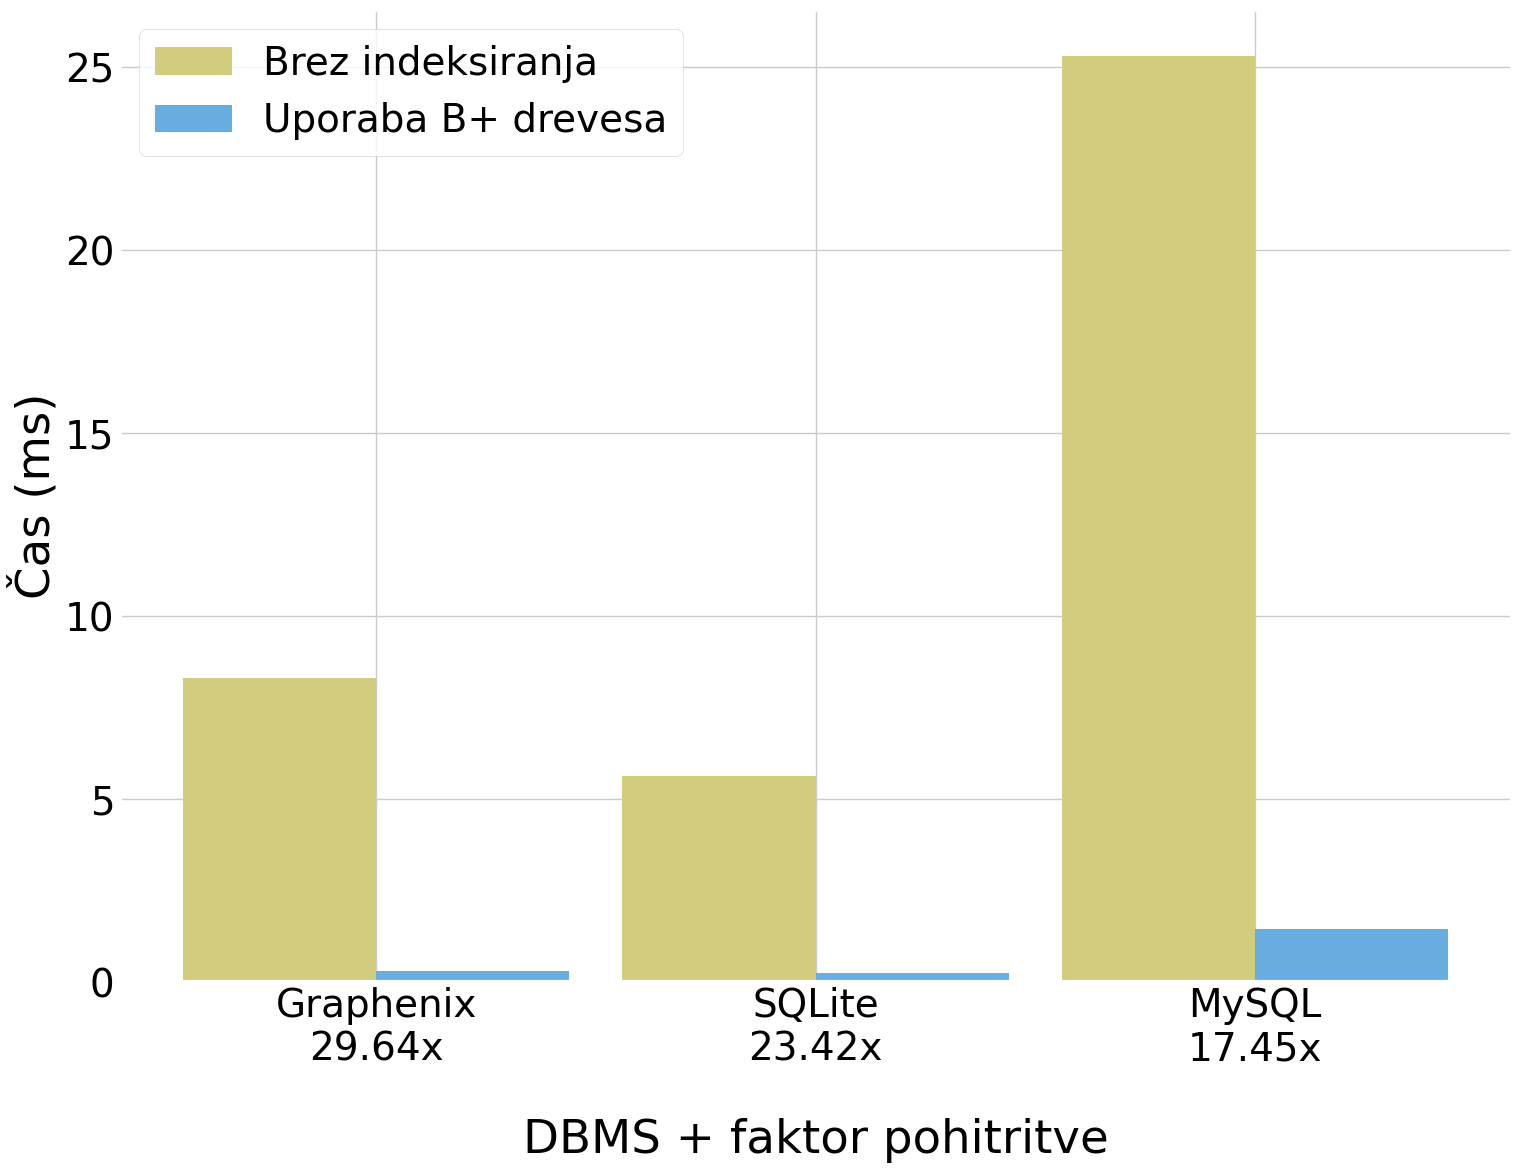
\includegraphics[height=4cm]{indexing_speedup_100000_v2.png}
                \caption*{Pohitritve s pomočjo indeksiranja po optimizaciji.}
            \end{minipage}
        \end{figure}
    \end{frame}

\section{Sklepne ugotovitve}
\begin{frame}
\frametitle{Sklepne ugotovitve}
    \begin{itemize}
        \item Kje je rešitev uporabna?
        \item Kaj rešitvi manjka za uporabo v produkcijskem okolju?
        \item Ali je bil razvoj uspešen?
    \end{itemize}
\end{frame}

\begin{frame}
\Huge{\centerline{Hvala za pozornost}}
\end{frame}

%----------------------------------------------------------------------------------------

\end{document} 